% ----------------------------------------------------------------------------------------------------- %
% Arquivo Principal - Trabalho de Sistemas Operacionais
% ----------------------------------------------------------------------------------------------------- %

\documentclass[tcc1]{classe_uftex/uftex}
\newcommand\uftex{UF\TeX}

\usepackage{lipsum}
\usepackage{tikz}
\usepackage[siunitx]{circuitikz}
\usetikzlibrary{arrows}
\usepackage{multirow}
\usepackage{graphicx}
\graphicspath{{images/}}
\usepackage{booktabs}

\usepackage[alf,abnt-emphasize=bf]{referencias_abnt/abntex2cite}
\renewcommand{\backrefpagesname}{}
\renewcommand{\backref}{}
\renewcommand*{\backrefalt}[4]{}

\makelosymbols
\makeloabbreviations

% ========================================================================= %
% PATCH DE CORREÇÃO
% ========================================================================= %
\makeatletter
\renewcommand\maketitle{%
  \ltx@ifpackageloaded{hyperref}{\uftex@hypersetup}{}%
 \begin{titlepage}
 \begin{center}
 
\includegraphics[scale=.3]{classe_uftex/logouft}\\
 \setstretch{1}
 \MakeUppercase{\bf\frontcover@maintext}
 \end{center}
  \begin{center}
  \vspace{4cm}
  \nohyphens{\MakeUppercase{\bf Henrique Noronha}}\par
  \nohyphens{\MakeUppercase{\bf Lauro Oliveira Mota}}\par
  \nohyphens{\MakeUppercase{\bf João Victor Melo do Nascimento}}\par
  \nohyphens{\MakeUppercase{\bf Hátilan Caio Alves Fontes}}\par
  \vspace{4cm}
  \nohyphens{\bf\MakeUppercase\local@title}\par
  \vfill
  {\bf\frontpage@bottomtext}
  \end{center}
  \end{titlepage}
  \global\let\maketitle\relax \global\let\and\relax
}

\renewcommand\makefrontpage{%
  \begin{center}
  {\bf Henrique Noronha}\par
  {\bf Lauro Oliveira Mota}\par
  {\bf João Victor Melo do Nascimento}\par
  {\bf Hátilan Caio Alves Fontes}\par
  \vfill
   \nohyphens{\bf \local@title}\par
  \end{center}
  \vfill
  \begin{flushright}
  \begin{minipage}{8.45cm}
  \setstretch{1}
  \frontpage@maintext
  \end{minipage}\par
 \end{flushright}
  \vfill
  \frontpage@bottomtext}

\renewcommand\frontpage@maintext{
  \sloppy\nohyphens{\local@doctype\ apresentado à \local@universityname\ para obten{\c c}{\~ a}o do t{\' i}tulo de \local@degname\ em \local@deptname .}
}

\renewenvironment{abstract}{%
\cleardoublepage \thispagestyle{empty} \chapter*{Resumo} \setlength{\parindent}{0pt}
}{\vspace{.5cm}
\count1=0
\noindent\nohyphens{{\bfseries Palavra-chave}:} \@whilenum \count1<\value{keywords} \do {%
        \nohyphens{\csname uftKeyword:\the\count1 \endcsname.}
        \advance\count1 by 1}\par}

\renewenvironment{foreignabstract}{%
\cleardoublepage \thispagestyle{empty} \chapter*{Abstract} \setlength{\parindent}{0pt}
}{\vspace{.5cm}
\noindent\nohyphens{{\bfseries Keywords}:}
\count1=0
    \@whilenum \count1<\@foreignkeyword \do{%
    \nohyphens{\protect\csname uftForeignkeyword:\the\count1\expandafter\endcsname .}
    \advance\count1 by 1}\par}

\def\@degreename{Bacharel}
\def\local@degname{Bacharel}
\def\local@deptname{Ciência da Computação}
\def\local@programname{Ciência da Computação}
\def\local@doctype{Relatório de Sistemas Operacionais}
\makeatother
% ========================================================================= %

\begin{document}

  \title{Análise Comparativa de Gerenciamento de Recursos do SO: Ableton Live vs. FL Studio}
  \author{Henrique}{Noronha Fernandes}
  \advisor{Prof.}{[Nome do Professor de SO]}{[Sobrenome]}{[Titulação]}

  \department{Ciência da Computação}
  \date{15}{04}{2026}

  \keyword{Sistemas Operacionais}
  \keyword{Escalonamento de Threads}
  \keyword{Gerenciamento de Memória}
  \keyword{Latência de Áudio}
  \keyword{Análise de Desempenho}

  \foreignkeyword{Operating Systems}
  \foreignkeyword{Thread Scheduling}
  \foreignkeyword{Memory Management}
  \foreignkeyword{Audio Latency}
  \foreignkeyword{Performance Analysis}

  \maketitle
  \frontmatter

  \printlosymbols
  \printloabbreviations
  \tableofcontents

\mainmatter
\onehalfspacing

% ----------------------------------------------------------------------------------------------------- %
\chapter{Introdução}

Os Sistemas Operacionais (SO) evoluíram bastante ao longo do tempo. Saíram
de monitores simples de execução sequencial e se tornaram sistemas
complexos, que precisam dar conta de hardware e software ao mesmo tempo.
Enquanto as primeiras gerações se preocupavam basicamente com a abstração
de comandos básicos e com a organização de arquivos, os sistemas atuais
precisam lidar com uma arquitetura de múltiplos núcleos (\textit{multicore}),
memória virtual e interrupções em escala de milissegundos. Nesse cenário,
muitos computadores pessoais acabam sendo usados como Estações de Trabalho
de Áudio Digital (DAWs, do inglês \textit{Digital Audio Workstations}). As
DAWs são softwares complexos, e a performance delas não depende só da força
bruta do processador, mas também de como o SO gerencia as \textit{threads},
aloca memória e cuida das operações de entrada e saída (I/O) em alta
velocidade.

O grande desafio desse tipo de aplicação é que ela precisa operar sob
restrições de tempo real. Segundo a classificação de
\citeonline{silberschatz2018}, as DAWs se enquadram como sistemas de
tempo real não crítico (\textit{soft real-time}). Isso quer dizer que um
atraso no atendimento de um processo não causa falha grave no computador,
mas atrapalha bastante a qualidade do serviço. No caso do áudio, isso se
manifesta como falhas e artefatos sonoros. Para evitar que isso aconteça,
o SO precisa garantir que as \textit{threads} de áudio tenham preferência
sobre os processos comuns, reduzindo a latência de despacho e a latência
de interrupção.

A partir disso, este trabalho faz uma análise comparativa do consumo e
do gerenciamento de recursos do SO entre duas das DAWs mais usadas no
mercado: o Ableton~Live e o FL~Studio. A ideia é mapear como cada
arquitetura afeta o consumo de CPU, o comportamento \textit{multithread},
o uso de memória RAM e a latência de I/O sob as mesmas condições de
estresse. Com isso, esperamos mostrar na prática como as decisões de
escalonamento e a arquitetura do SO impactam ambientes de alta exigência
em tempo real.


% ----------------------------------------------------------------------------------------------------- %
\chapter{Referencial Teórico}

\section{Gerenciamento de Processos e \textit{Threads}}

Um processo é um programa que está sendo executado pelo sistema operacional,
com espaço de endereçamento próprio e os recursos atribuídos pelo SO
\cite{silberschatz2018}. Dentro de um mesmo processo podem existir várias
\textit{threads}: unidades menores de execução que compartilham o espaço de
endereçamento do processo, mas têm pilha e registradores próprios
\cite{tanenbaum2016}. Como elas compartilham memória, a troca de contexto
entre \textit{threads} é bem mais barata do que entre processos. Por causa
disso, motores de áudio costumam usar \textit{multithreading} para dividir o
processamento de blocos de amostras entre os núcleos do hardware.

\subsection{Escalonador do Windows NT}

O escalonador do Windows NT é preemptivo e baseado em prioridades, com
32 níveis numerados de 0 a 31. Os níveis 1 a 15 formam a faixa de usuário e
os níveis 16 a 31 formam a faixa de tempo real \cite{stallings2017os}. Os
valores observados nos testes deste trabalho ficam todos na faixa de
usuário: \textit{Normal} (8), \textit{Above Normal} (10) e \textit{High}
(12 e 13).

Cada \textit{thread} tem uma prioridade base, derivada da classe do processo.
Em tempo de execução, o sistema pode aplicar um \textit{priority boost}
temporário para evitar \textit{starvation} ou premiar \textit{threads} que
acabaram de acordar de uma operação de I/O \cite{stallings2017os}. Esse
\textit{boost} vai caindo até a \textit{thread} voltar à prioridade base, e
isso explica por que o Process Explorer mostra valores diferentes para
prioridade base e prioridade dinâmica.

\subsection{Tempo Real Crítico vs.\ Não Crítico}

\citeonline{silberschatz2018} dividem os sistemas de tempo real em dois
tipos. No tempo real crítico (\textit{hard real-time}), perder um prazo é
uma falha grave, inaceitável em aplicações como aviônica ou equipamento
médico. No tempo real não crítico (\textit{soft real-time}), perder um prazo
eventualmente atrapalha a qualidade do serviço, mas não compromete o sistema
como um todo.

As DAWs ficam nesse segundo grupo. Quando um \textit{buffer} de áudio não é
preenchido a tempo, o usuário ouve um \textit{dropout}, mas a máquina
continua estável. Para garantir prioridade sem precisar de garantia formal,
basta colocar as \textit{threads} de áudio em prioridade maior que a dos
processos comuns. Assim, o escalonador as despacha primeiro quando há
disputa por CPU.


\section{Interrupções e Latência de I/O em Tempo Real}

Uma interrupção de hardware é um sinal assíncrono que um periférico envia
ao processador para avisar que precisa de atenção imediata
\cite{silberschatz2018}. Quando o sinal chega, o processador para a
\textit{thread} que está executando, salva seu estado e transfere o
controle para a Rotina de Serviço de Interrupção (ISR). O intervalo entre o
sinal e o início da ISR é chamado de latência de interrupção. Somando esse
intervalo ao tempo de troca de contexto até a \textit{thread} destino, temos
a latência de despacho \cite{stallings2017os}. No caso do áudio, se essa
latência ultrapassar o período do \textit{buffer}, aparece silêncio ou
artefato sonoro na saída.

\subsection{\textit{Callback} de Áudio e Tamanho de \textit{Buffer}}

Drivers de áudio modernos funcionam no modelo \textit{pull callback}: o
hardware solicita periodicamente um bloco de $N$ amostras, e o motor de
áudio precisa entregá-lo antes do próximo bloco ser pedido \cite{fons2010}.
A relação entre tamanho do \textit{buffer} e latência é dada por:

\begin{equation}
  L = \frac{N}{f_s}
\end{equation}

\noindent onde $L$ é a latência em segundos, $N$ o tamanho do bloco em
amostras e $f_s$ a taxa de amostragem. Por exemplo, com $f_s = 44.100$~Hz e
$N = 256$, a latência fica em torno de $5{,}8$~ms. Reduzir $N$ diminui a
latência percebida, mas aumenta a frequência das interrupções e, com isso, a
carga sobre o escalonador \cite{kim2003}.

\subsection{ASIO vs.\ WDM/DirectSound}

O Windows oferece dois caminhos principais para áudio. No caminho
WDM/DirectSound, o sinal passa pelo \textit{Kernel Audio Mixer} (KMixer),
que junta os fluxos de vários aplicativos antes de enviar para o hardware
\cite{microsoft2023asio}. Como o KMixer precisa ser acordado a cada ciclo
de \textit{buffer}, isso acaba adicionando latência e gerando interrupções
extras.

Já o protocolo ASIO (\textit{Audio Stream Input/Output}) dá ao driver do
fabricante acesso direto ao hardware, pulando o KMixer
\cite{microsoft2023asio}. O resultado é menos latência e menos pressão sobre
o escalonador.

\subsection{Algoritmos Formais de Escalonamento em Tempo Real}

Vale lembrar que existe uma linha de pesquisa formal sobre escalonamento de
prazos em tempo real. \citeonline{liu1973} formalizaram o problema com o
algoritmo \textit{Rate Monotonic}, e \citeonline{buttazzo2011} mostraram que
garantir prazos formalmente exige análise de pior caso (WCET). As DAWs, por
serem \textit{soft real-time}, não usam esse rigor. Elas apenas aumentam a
prioridade das \textit{threads} de áudio no escalonador comum do SO,
abrindo mão da garantia formal em troca de simplicidade de implementação.


\section{Gerenciamento de Memória e Paginação}

Cada processo recebe do SO um espaço de endereçamento virtual contíguo e
isolado, independente da memória física disponível \cite{silberschatz2018}.
A tradução entre endereço virtual e físico é feita pela MMU, usando as
tabelas de páginas mantidas pelo \textit{kernel}. Na paginação por demanda,
uma página só é mapeada para um quadro físico (\textit{frame}) quando é
acessada pela primeira vez. Esse evento é chamado de falta de página
(\textit{page fault}) \cite{tanenbaum2016}. Para resolver uma falta de
página, o \textit{kernel} suspende a \textit{thread}, localiza a página (ou
lê do disco se necessário) e retoma a execução. O tempo total dessa
operação é não determinístico e pode variar de microssegundos a
milissegundos, dependendo de onde a página estava.

Para áudio em tempo real, uma falta de página no meio do processamento de
um bloco é especialmente cara: a \textit{thread} fica bloqueada esperando o
\textit{kernel} resolver, enquanto o prazo do \textit{buffer} continua
correndo \cite{kim2003}. Sistemas críticos resolvem esse problema fixando
páginas na RAM com \texttt{mlock()} no Linux ou \texttt{VirtualLock()} no
Windows. As DAWs comerciais costumam adotar uma estratégia diferente:
alocam boa parte da memória logo na inicialização, o que tem efeito
parecido na prática.

\subsection{\textit{Eager} vs.\ \textit{Lazy Allocation}}

\citeonline{tanenbaum2016} contrastam dois modelos de alocação. Na
\textit{eager allocation}, o processo reserva e inicializa toda a memória
prevista logo no início. Isso elimina faltas de página no caminho crítico,
mas mantém uma pegada de memória grande mesmo em repouso. Já na
\textit{lazy allocation}, os recursos são alocados só conforme vão sendo
demandados; a pegada em repouso fica mínima, mas pode haver latência não
determinística no momento da primeira alocação. Como será discutido no
Capítulo~5, esse contraste aparece de forma bem clara nos resultados deste
trabalho.

\subsection{\textit{Private Bytes}}

O contador \textit{Private Bytes} do Windows mede a memória virtual
comprometida exclusivamente pelo processo, sem contar DLLs e outras regiões
compartilhadas \cite{stallings2018}. Essa é a métrica que melhor reflete o
custo real de memória da aplicação, já que mostra o que precisaria ser
paginado para disco caso o sistema ficasse sem RAM física. No caso das
DAWs, o crescimento desse contador ao carregar trilhas vem principalmente
dos \textit{buffers} de pré-leitura e das estruturas de decodificação que
precisam ficar em memória para garantir reprodução de baixa latência.


% ----------------------------------------------------------------------------------------------------- %
\chapter{Metodologia}

O estudo adota uma abordagem quantitativa e comparativa para analisar o
gerenciamento de recursos de \textit{Digital Audio Workstations} (DAWs)
sob a ótica de Sistemas Operacionais. O foco é a interação entre o
\textit{kernel} do Windows~11 (build~26200, x64) e os motores de áudio do
Ableton~Live~12 e do FL~Studio~24. Os experimentos foram feitos em um
notebook ASUS Vivobook K3605ZF com processador Intel Core i5-12500H
(12~núcleos, 16~\textit{threads}, base 3,1~GHz), 16~GB de RAM DDR4 e GPU
NVIDIA (driver \texttt{nvlddmkm.sys} v581.29). Para preservar as escolhas
arquiteturais nativas de cada fabricante, o FL~Studio rodou com o driver
FL~Studio ASIO e o Ableton~Live rodou com MME/DirectX. O \textit{Fruity
Limiter} do canal Master do FL~Studio foi removido antes dos testes para
manter paridade na cadeia de sinal. O Windows Defender ficou ativo em
todas as sessões, em condições iguais para as duas DAWs.

A coleta de dados foi feita com três ferramentas complementares. O
Performance Monitor (PerfMon) capturou contadores do \textit{kernel} a
1~Hz, especificamente \texttt{\% Tempo de Processador},
\texttt{Private Bytes} e \texttt{Contagem de Threads} por processo, e os
dados foram exportados via \texttt{relog} para o formato \texttt{.csv}
\cite{microsoft2023perfmon}. O Process Explorer (Sysinternals) foi
usado para inspecionar as \textit{threads} individuais, suas prioridades
de escalonamento e o consumo de CPU por unidade de execução. O
LatencyMon v7.31 \cite{asio4all} mediu a latência
\textit{interrupt-to-process}, os tempos de rotinas DPC e ISR e a
contagem de \textit{hard pagefaults} no nível do sistema.

O protocolo experimental foi composto por cinco testes sequenciais. O
Teste~1, de repouso, coletou dados durante 2,5~minutos com a DAW aberta
e sem projeto carregado. O Teste~2, de carga \textit{I/O-bound},
adicionou a reprodução simultânea em \textit{loop} de 20~trilhas AIFF
(PCM não comprimido) por 3~minutos. No Teste~3, de escalonamento, o
Process Explorer foi usado para inspecionar a composição, a prioridade e
a distribuição das \textit{threads} com o projeto ativo. No Teste~4, de
latência, o LatencyMon foi executado por 2~min~50~s sobre o mesmo
projeto, registrando DPCs, ISRs e \textit{pagefaults}. Por fim, no
Teste~5, de estresse CPU-bound, foram inseridas cinco instâncias do
reverb nativo de cada DAW no canal Master, e o tamanho do \textit{buffer}
foi reduzido aos poucos de 4096 até 128~\textit{samples}. O ponto de
ruptura (\textit{buffer underrun}) foi identificado pelo aparecimento de
\textit{dropouts} audíveis.


% ----------------------------------------------------------------------------------------------------- %
\chapter{Resultados}

\section{Testes 1 e 2: consumo em repouso e carga I/O-bound}

Os Testes~1 e~2 avaliaram o comportamento de CPU, memória e
\textit{threads} em dois cenários consecutivos: DAW em repouso (sem projeto)
e com reprodução simultânea de 20~trilhas AIFF em \textit{loop}. Os dados,
amostrados a 1~Hz via PerfMon durante 2,5 e 3~minutos respectivamente, estão
consolidados nas Tabelas~\ref{tab:t1} e~\ref{tab:t2}.

\begin{table}[ht]
\centering
\caption{Resumo estatístico do Teste~1 (repouso) e do Teste~2 (20 trilhas AIFF).}
\label{tab:t1}
\begin{tabular}{llcccc}
\toprule
\textbf{Teste} & \textbf{Métrica} & \textbf{DAW} & \textbf{Mín.} & \textbf{Média} & \textbf{Máx.} \\
\midrule
\multirow{6}{*}{T1: repouso}
  & \multirow{2}{*}{\% CPU}
    & Ableton Live 12  & 0{,}00\% & 10{,}95\% & 33{,}73\% \\
  & & FL Studio (FL64) & 0{,}00\% & 12{,}38\% & 37{,}72\% \\
\cmidrule{2-6}
  & \multirow{2}{*}{Private Bytes (MB)}
    & Ableton Live 12  & 338{,}6 & 536{,}8 & 538{,}3 \\
  & & FL Studio (FL64) &  95{,}6 &  95{,}8 &  95{,}8 \\
\cmidrule{2-6}
  & \multirow{2}{*}{Threads ativas}
    & Ableton Live 12  &  8 & 54{,}8 & 56 \\
  & & FL Studio (FL64) & 44 & 44{,}0 & 45 \\
\midrule
\multirow{6}{*}{T2: 20 trilhas}
  & \multirow{2}{*}{\% CPU}
    & Ableton Live 12  & 0{,}00\% &  3{,}74\% & 20{,}11\% \\
  & & FL Studio (FL64) & 0{,}00\% &  4{,}80\% & 31{,}16\% \\
\cmidrule{2-6}
  & \multirow{2}{*}{Private Bytes (MB)}
    & Ableton Live 12  & 601{,}6 & 601{,}7 & 604{,}5 \\
  & & FL Studio (FL64) & 137{,}6 & 147{,}6 & 147{,}6 \\
\cmidrule{2-6}
  & \multirow{2}{*}{Threads ativas}
    & Ableton Live 12  & 54 & 55{,}3 & 56 \\
  & & FL Studio (FL64) & 26 & 27{,}0 & 28 \\
\bottomrule
\multicolumn{6}{l}{\footnotesize Fonte: dados coletados pelos autores via PerfMon, 26 maio 2026.}
\end{tabular}
\end{table}

Em repouso, o FL~Studio consumiu CPU média um pouco maior que o
Ableton~Live ($12{,}38\%$ contra $10{,}95\%$). Por outro lado, o
Ableton~Live alocou $5{,}6$ vezes mais memória ($536{,}8$~MB contra
$95{,}8$~MB) e manteve quase o dobro de \textit{threads} ativas
($54{,}8$ contra $44{,}0$). Com as 20~trilhas em reprodução, as duas DAWs
reduziram o consumo médio de CPU: o Ableton caiu de $10{,}95\%$ para
$3{,}74\%$ e o FL~Studio caiu de $12{,}38\%$ para $4{,}80\%$. A memória
cresceu de forma moderada, $+64{,}9$~MB no Ableton e $+51{,}8$~MB no
FL~Studio. O FL~Studio reduziu suas \textit{threads} de 44 para 27 ao
carregar o projeto, uma queda de $38\%$, enquanto o Ableton praticamente
não mudou ($54{,}8$ para $55{,}3$). As Figuras~\ref{fig:t1cpu}
até~\ref{fig:t2thr} mostram esses comportamentos.

\begin{figure}[ht]
\centering
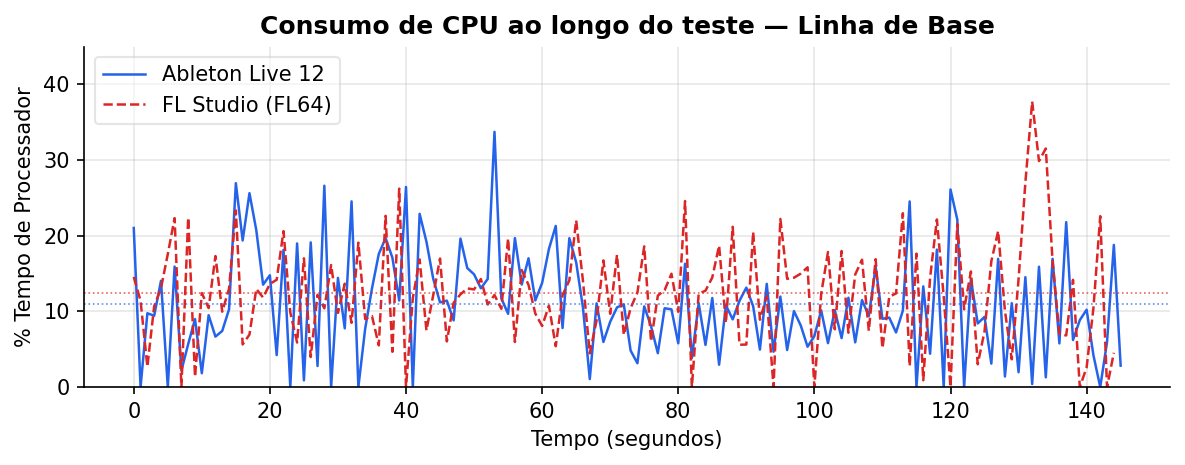
\includegraphics[width=0.95\textwidth]{grafico_cpu}
\caption{Consumo de CPU em repouso no Teste 1.}
\label{fig:t1cpu}
\par\footnotesize{Fonte: dados coletados pelos autores via PerfMon, 26 maio 2026.}
\end{figure}

\begin{figure}[ht]
\centering
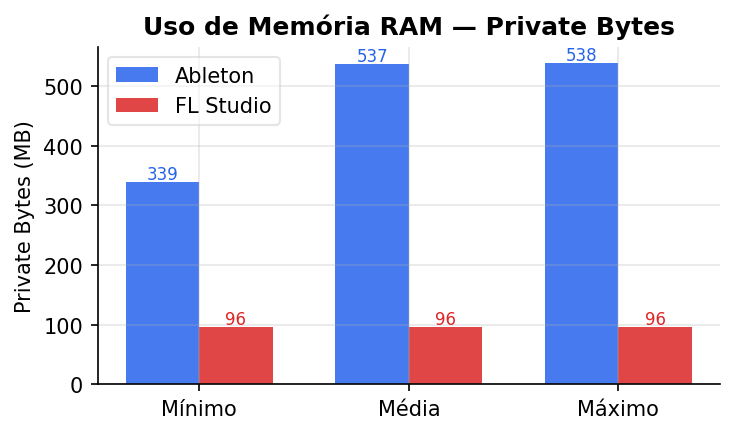
\includegraphics[width=0.48\textwidth]{grafico_ram}
\hfill
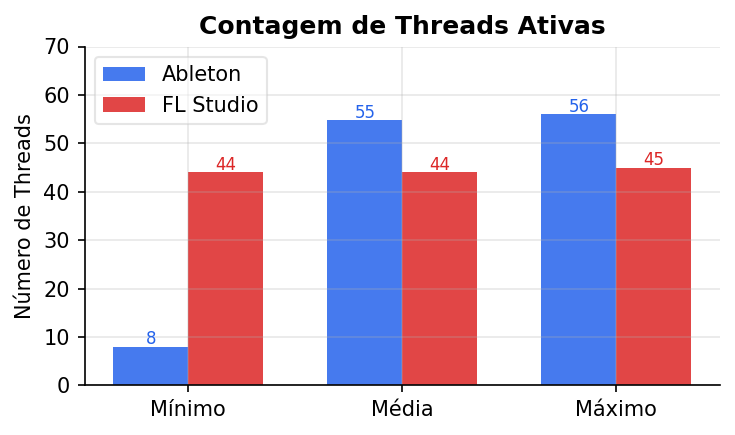
\includegraphics[width=0.48\textwidth]{grafico_threads}
\caption{Uso de RAM (\textit{Private Bytes}) e número de \textit{threads} em repouso no Teste 1.}
\label{fig:t1ram}
\par\footnotesize{Fonte: dados coletados pelos autores via PerfMon, 26 maio 2026.}
\end{figure}

\begin{figure}[ht]
\centering
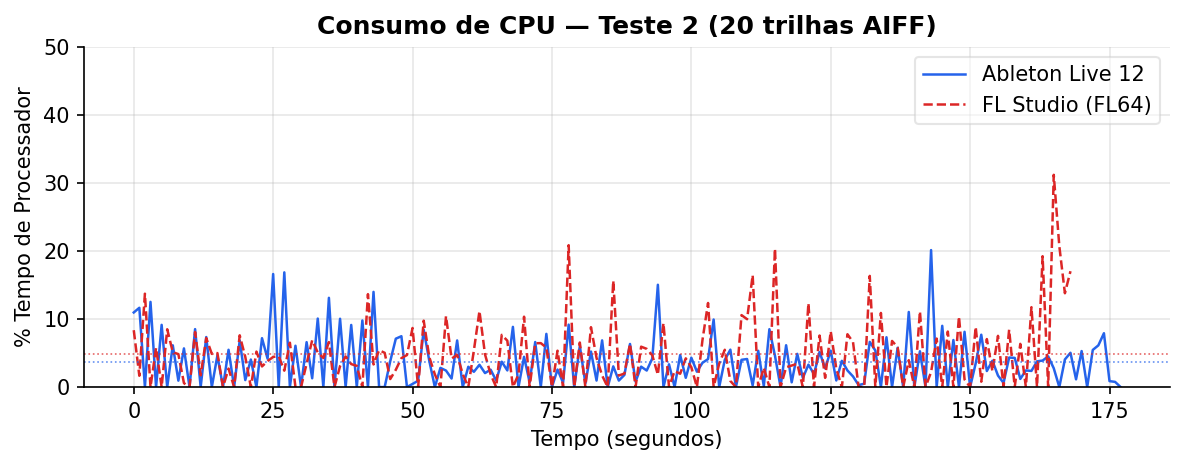
\includegraphics[width=0.95\textwidth]{t2_grafico_cpu}
\caption{Consumo de CPU durante a reprodução de 20 trilhas AIFF no Teste 2.}
\label{fig:t2cpu}
\par\footnotesize{Fonte: dados coletados pelos autores via PerfMon, 26 maio 2026.}
\end{figure}

\begin{figure}[ht]
\centering
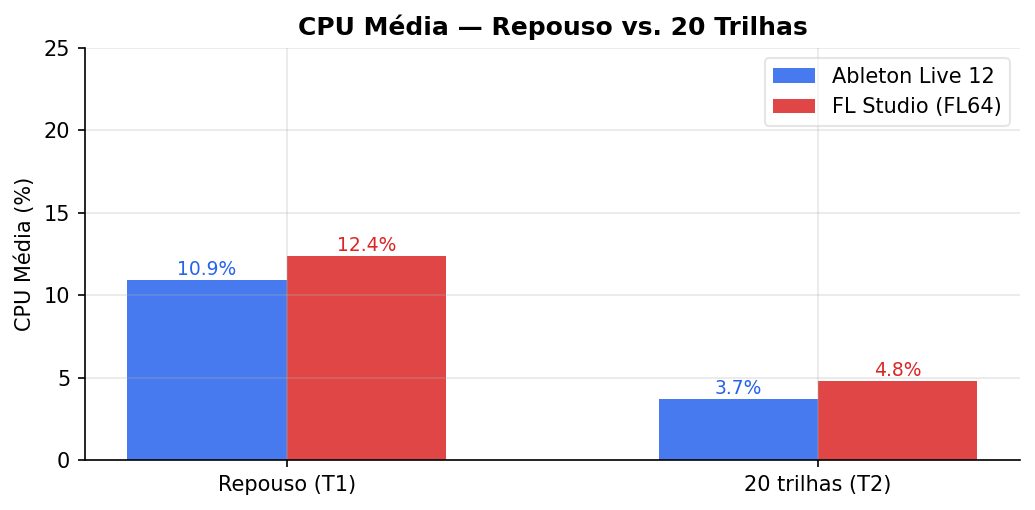
\includegraphics[width=0.48\textwidth]{t2_cpu_comparativo}
\hfill
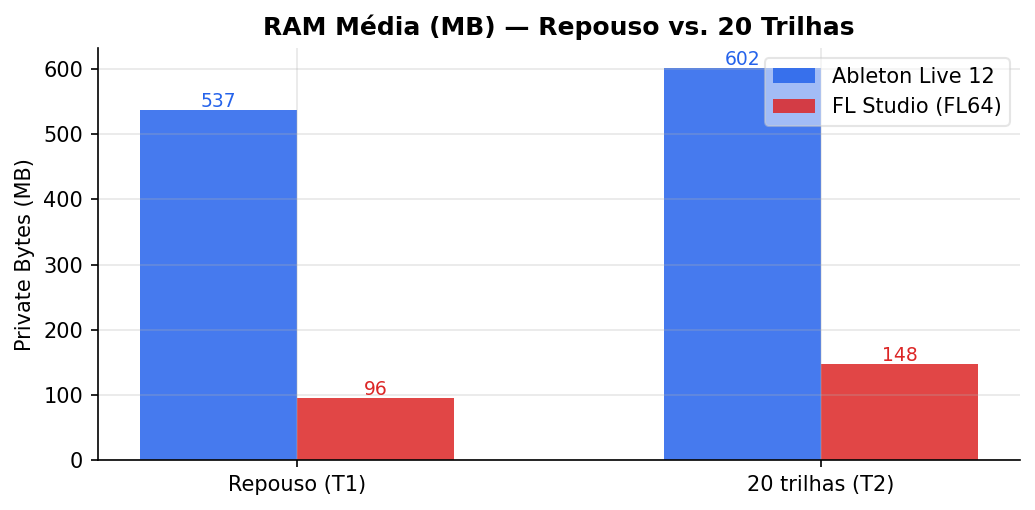
\includegraphics[width=0.48\textwidth]{t2_ram_comparativo}
\caption{Comparação de CPU e RAM médias entre repouso (T1) e 20 trilhas (T2).}
\label{fig:t2cpucomp}
\par\footnotesize{Fonte: dados coletados pelos autores via PerfMon, 26 maio 2026.}
\end{figure}

\begin{figure}[ht]
\centering
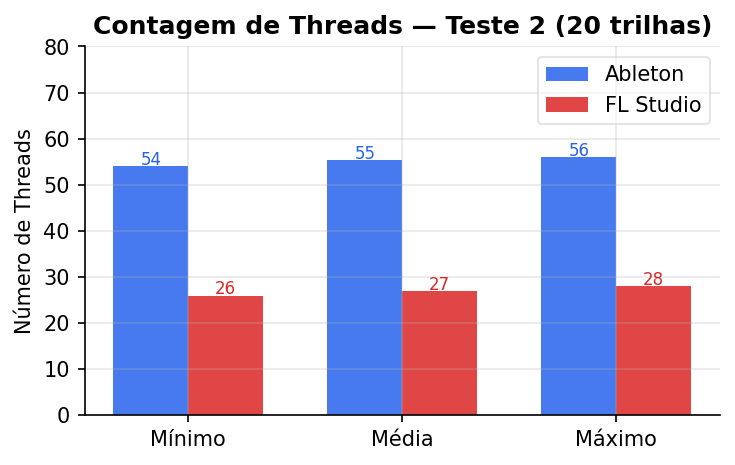
\includegraphics[width=0.65\textwidth]{t2_grafico_threads}
\caption{Número de \textit{threads} ativas com 20 trilhas em reprodução no Teste 2.}
\label{fig:t2thr}
\par\footnotesize{Fonte: dados coletados pelos autores via PerfMon, 26 maio 2026.}
\end{figure}

% ---------------------------------------------------------------- %
\section{Teste 3: escalonamento de threads}

A inspeção via Process Explorer com o projeto em reprodução mostrou
diferenças relevantes na composição e na prioridade das \textit{threads}
(Tabela~\ref{tab:t3}). O FL~Studio opera com prioridade base~10
(\textit{Above Normal}) e dinâmica~12 (\textit{High}), enquanto o
Ableton~Live opera com base~8 (\textit{Normal}) e dinâmica~10. Nenhuma das
duas atingiu o nível \textit{Time Critical} (15). Quanto à composição, 14
das 29~\textit{threads} do FL~Studio pertencem ao módulo
\texttt{QuickFontCache}, que cuida da renderização da interface, e só 5
estão associadas ao \texttt{FLEngine\_x64}, que é o motor de áudio. No
Ableton~Live, cerca de 30 das 55~\textit{threads} vêm do
\texttt{ucrtbase.dll}, que é o \textit{thread pool} do C runtime. As
Figuras~\ref{fig:t3prio} e~\ref{fig:t3comp} detalham esses dados.

\begin{table}[ht]
\centering
\caption{Composição e prioridade das \textit{threads} no Teste 3, obtidas via Process Explorer.}
\label{tab:t3}
\begin{tabular}{lcc}
\toprule
\textbf{Parâmetro} & \textbf{FL Studio (FL64)} & \textbf{Ableton Live 12} \\
\midrule
Total de \textit{threads}           & 29                & 55                \\
Prioridade base (thread principal)  & 10 (Above Normal) & 8 (Normal)        \\
Prioridade dinâmica                 & 12 (High)         & 10 (Above Normal) \\
CPU da thread principal             & 0{,}93\%          & 0{,}75\%          \\
Thread \textit{Time Critical} (15)? & Não               & Não               \\
Módulo dominante                    & QuickFontCache    & ucrtbase          \\
Thread de driver de áudio           & ilwasapi2asio\_x64& DSOUND.dll        \\
\bottomrule
\multicolumn{3}{l}{\footnotesize Fonte: dados coletados pelos autores via Process Explorer, 26 maio 2026.}
\end{tabular}
\end{table}

\begin{figure}[ht]
\centering
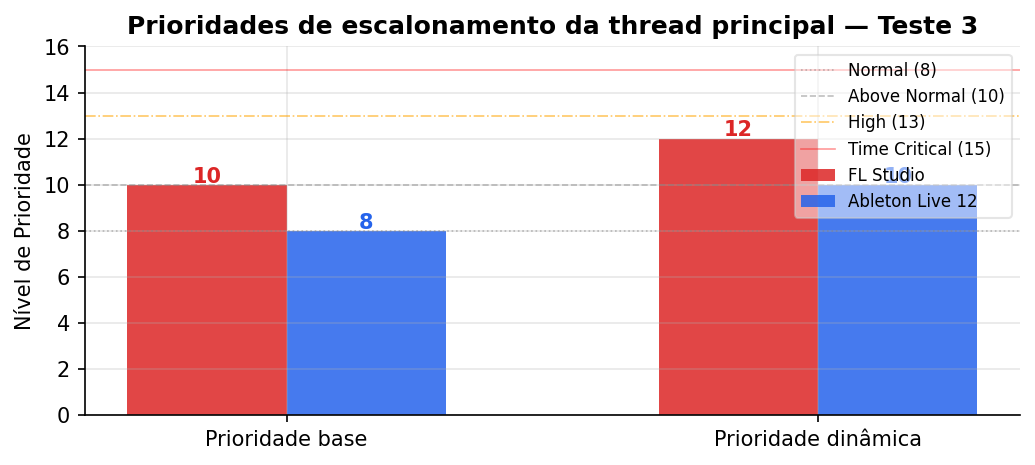
\includegraphics[width=0.75\textwidth]{t3_prioridades}
\caption{Prioridades de escalonamento da \textit{thread} principal no Teste 3.}
\label{fig:t3prio}
\par\footnotesize{Fonte: dados coletados pelos autores via Process Explorer, 26 maio 2026.}
\end{figure}

\begin{figure}[ht]
\centering
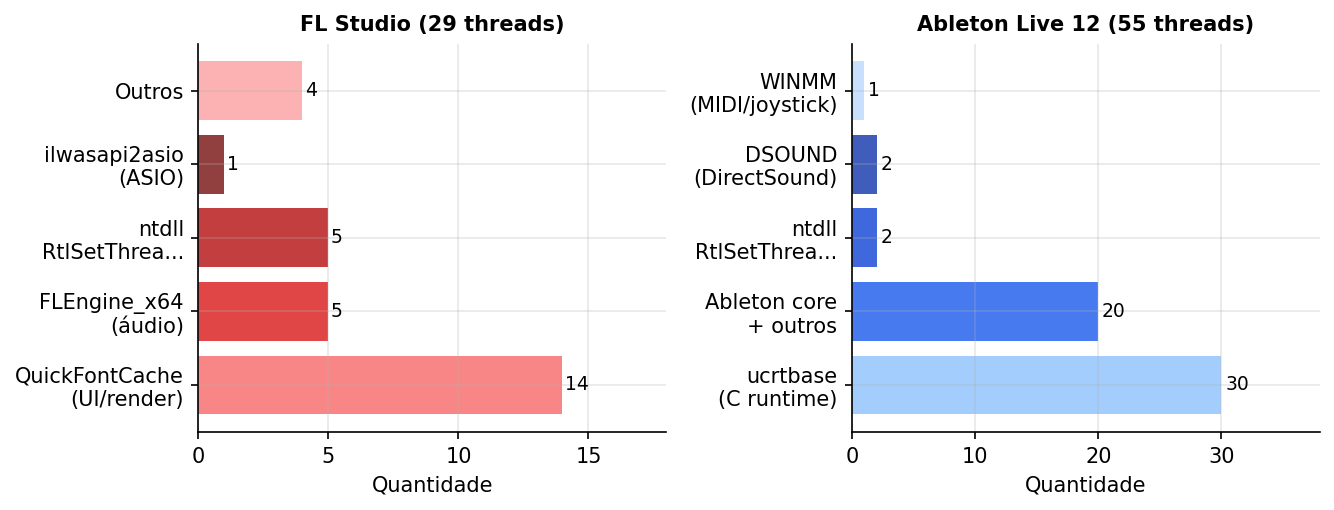
\includegraphics[width=0.95\textwidth]{t3_composicao_threads}
\caption{Distribuição das \textit{threads} por módulo no Teste 3.}
\label{fig:t3comp}
\par\footnotesize{Fonte: dados coletados pelos autores via Process Explorer, 26 maio 2026.}
\end{figure}

% ---------------------------------------------------------------- %
\section{Teste 4: latência com driver nativo}

O LatencyMon classificou o sistema como apto nas duas DAWs
(Tabela~\ref{tab:t4}). A latência máxima \textit{interrupt-to-process} foi
de $805{,}40\,\mu$s no Ableton~Live e $939{,}80\,\mu$s no FL~Studio, ambas
dentro do limite aceitável de $1000\,\mu$s. O maior DPC do FL~Studio veio
do driver NVIDIA \texttt{nvlddmkm.sys} ($647{,}07\,\mu$s). Em ambas as
sessões, o processo com mais \textit{hard pagefaults} foi o
\texttt{msmpeng.exe} do Windows Defender. O FL~Studio teve percentual de
CPU em DPCs um pouco maior ($0{,}090\%$ contra $0{,}074\%$) e em ISRs
($0{,}044\%$ contra $0{,}023\%$).

\begin{table}[ht]
\centering
\caption{Resultados de latência do Teste 4, obtidos com o LatencyMon v7.31.}
\label{tab:t4}
\begin{tabular}{lcc}
\toprule
\textbf{Métrica} & \textbf{Ableton Live 12} & \textbf{FL Studio (FL64)} \\
\midrule
Conclusão do sistema                  & Apto               & Apto               \\
Latência máx. int.-to-proc. ($\mu$s)  & 805{,}40           & 939{,}80           \\
Latência méd. int.-to-proc. ($\mu$s)  &   8{,}50           &  16{,}96           \\
DPC máximo ($\mu$s)                   & 449{,}81           & 647{,}07           \\
ISR máximo ($\mu$s)                   & 267{,}52           & 401{,}24           \\
Tempo total em DPCs (\%)              & 0{,}074            & 0{,}090            \\
Tempo total em ISRs (\%)              & 0{,}023            & 0{,}044            \\
\textit{Hard pagefaults} totais       & 306                & 378                \\
Driver com maior DPC                  & \texttt{tcpip.sys} & \texttt{nvlddmkm.sys} \\
\bottomrule
\multicolumn{3}{l}{\footnotesize Fonte: dados coletados pelos autores via LatencyMon v7.31, 26 maio 2026.}
\end{tabular}
\end{table}





% ---------------------------------------------------------------- %
\section{Teste 5: estresse CPU-bound e ponto de ruptura}

Com cinco instâncias de reverb ativas no canal Master e as 20~trilhas em
reprodução, o tamanho do \textit{buffer} foi reduzido aos poucos até começar
a aparecer \textit{dropouts} audíveis (Tabela~\ref{tab:t5}). O FL~Studio
(ASIO) se manteve estável até $256$~\textit{samples} ($6$~ms) e quebrou em
$128$~\textit{samples}. O Ableton~Live (MME/DirectX) começou a apresentar
problemas já em $1024$~\textit{samples} ($23{,}2$~ms), com degradação cada
vez maior nos valores menores. As Figuras~\ref{fig:t5lat} e~\ref{fig:t5comp}
resumem esse comportamento.

\begin{table}[ht]
\centering
\caption{Ponto de ruptura observado no Teste 5 (estresse CPU-bound).}
\label{tab:t5}
\begin{tabular}{lccc}
\toprule
\textbf{Buffer (smp)} & \textbf{Latência (ms)} &
\textbf{FL Studio (ASIO)} & \textbf{Ableton (MME/DirectX)} \\
\midrule
4096 & 92{,}9 & ---                     & Estável         \\
2048 & 46{,}4 & ---                     & Estável         \\
1024 & 23{,}2 & ---             & Glitch         \\
 512 & 11{,}6 & Estável         & Glitch piora   \\
 384 &  9{,}0 & Estável         & ---            \\
 256 &  5{,}8 & Mínimo estável  & Glitch forte   \\
 128 &  2{,}9 & Glitch          & ---            \\
\bottomrule
\multicolumn{4}{l}{\footnotesize Fonte: dados coletados pelos autores, 27 maio 2026.}
\end{tabular}
\end{table}

\begin{figure}[ht]
\centering
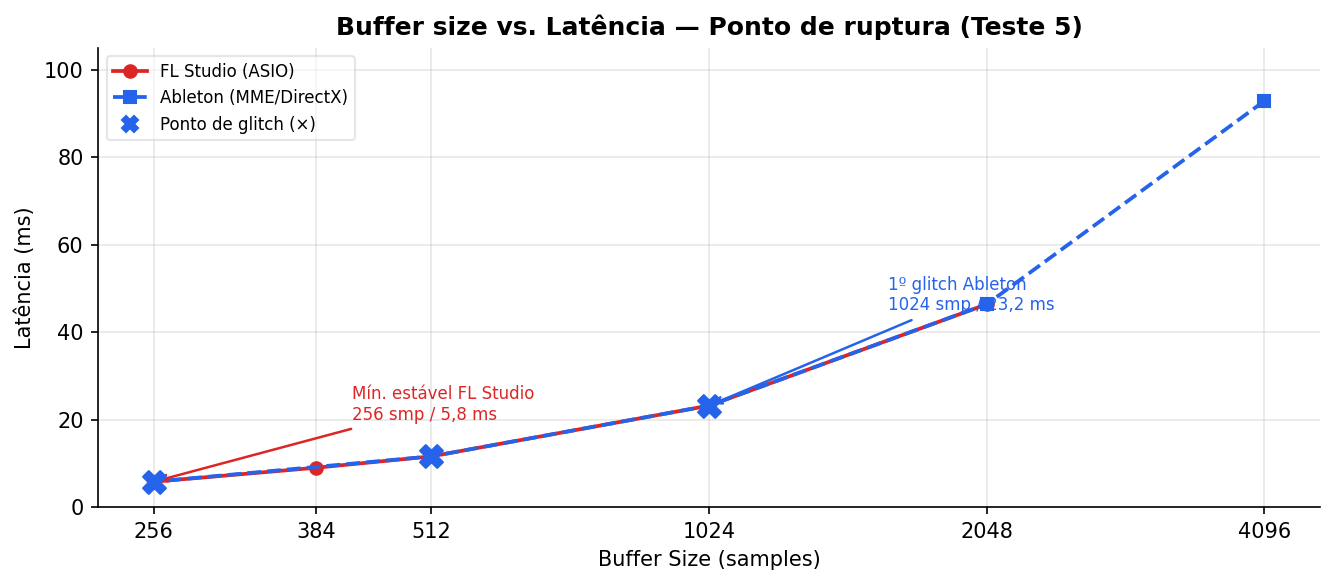
\includegraphics[width=0.95\textwidth]{t5_buffer_latencia}
\caption{Tamanho do \textit{buffer} e latência correspondente no Teste 5. O marcador $\times$ indica o ponto de \textit{dropout} em cada DAW.}
\label{fig:t5lat}
\par\footnotesize{Fonte: dados coletados pelos autores, 27 maio 2026.}
\end{figure}

\begin{figure}[!htb]
\centering
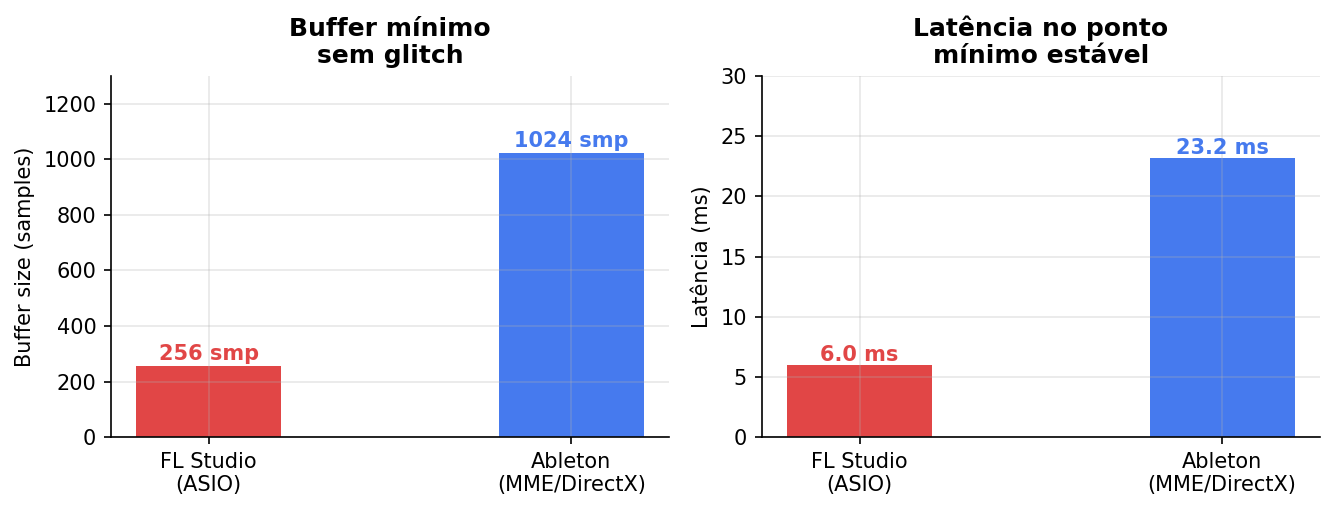
\includegraphics[width=0.65\textwidth,keepaspectratio]{t5_ruptura_comparativo}
\caption{Buffer mínimo estável e latência correspondente no Teste 5.}
\label{fig:t5comp}
\par\footnotesize{Fonte: dados coletados pelos autores, 27 maio 2026.}
\end{figure}

% ----------------------------------------------------------------------------------------------------- %

\chapter{Discussão}

\section{Análise do Teste 1 (repouso)}

Os resultados do Teste~1 mostram que as duas DAWs partem de pontos de
inicialização bem diferentes. O Ableton~Live segue a estratégia de
\textit{eager allocation}: aloca memória e cria \textit{threads} logo na
inicialização (cerca de 537~MB e 55~\textit{threads}), o que mantém a
latência de despacho baixa desde o início \cite{silberschatz2018}. O
FL~Studio adota \textit{lazy allocation} e mantém só o essencial em repouso
(cerca de 96~MB e 44~\textit{threads}), deixando para alocar mais recursos
só quando o projeto for carregado \cite{tanenbaum2016}.

\section{Análise do Teste 2 (20 trilhas AIFF)}

O Teste~2 trouxe três pontos interessantes. Primeiro, a redução de CPU sob
carga \textit{I/O-bound} nas duas DAWs pode ser explicada pelo driver de
áudio nativo: quando ele assume o controle exclusivo do hardware, acaba
eliminando a sobrecarga do \textit{Kernel Mixer} do Windows. Segundo, o
crescimento de RAM foi parecido em termos absolutos ($+65$~MB no Ableton
e $+52$~MB no FL~Studio), o que indica que o custo por trilha AIFF é
parecido nas duas arquiteturas. Terceiro, a queda de \textit{threads} no
FL~Studio (de 44 para 27) sugere que o motor de áudio consolida
\textit{threads} genéricas em outras mais especializadas quando o projeto
é carregado \cite{stallings2017os}.

\section{Análise do Teste 3 (escalonamento de threads)}

O FL~Studio opera com prioridade mais alta (base~10 e dinâmica~12), o que
em tese deveria garantir maior fatia de CPU em situações de disputa
\cite{silberschatz2018}. Mas, das 29~\textit{threads} totais, 14
pertencem ao \texttt{QuickFontCache}, ou seja, parte desse orçamento de
CPU é consumida pela interface gráfica, e não pelo motor de áudio. O
Ableton~Live, mesmo com prioridade base menor (8), distribui sua carga em
55~\textit{threads} usando o \textit{thread pool} do \texttt{ucrtbase}, o
que favorece a escalabilidade nos 16~\textit{threads} lógicos do
i5-12500H \cite{tanenbaum2016}. Vale notar que nenhuma das duas DAWs usa
prioridade \textit{Time Critical} (15), o que confirma o enquadramento
delas como sistemas \textit{soft real-time} \cite{stallings2017os}.

\section{Análise do Teste 4 (latência)}

O Teste~4 foi feito em um ambiente controlado, com o navegador e outros
aplicativos secundários fechados. O LatencyMon classificou as duas DAWs
como aptas para operação de áudio em tempo real. O Ableton~Live teve
latência máxima de $805\,\mu$s e o FL~Studio de $939\,\mu$s, uma diferença
de cerca de $17\%$, com ambas ficando abaixo do limite crítico de
$1000\,\mu$s definido pelo LatencyMon.

O principal fator de latência no FL~Studio foi o driver NVIDIA
\texttt{nvlddmkm.sys}, que gerou o DPC máximo de $647\,\mu$s. Isso indica
que a GPU do sistema gera interrupções de duração mais alta e acaba
disputando o escalonador com o motor de áudio, independentemente da DAW
em uso \cite{silberschatz2018}. No Ableton~Live, o maior DPC veio do
\texttt{tcpip.sys}, o que sugere que o subsistema gráfico estava
pressionando menos o escalonador durante essa sessão específica.

Esse resultado contrasta com uma sessão anterior do FL~Studio que foi
feita com o Windows Defender em surto de varredura. Nessa sessão a latência
chegou a $5274\,\mu$s e a conclusão do LatencyMon foi de não apto. A
comparação entre as duas sessões mostra que interferências de processos
externos, principalmente antivírus e drivers de GPU, podem ter impacto
determinante na estabilidade de áudio em tempo real, às vezes até maior
do que as próprias diferenças entre as arquiteturas das DAWs
\cite{tanenbaum2016}. Em condições equivalentes, as duas aplicações
parecem igualmente capazes de operar sem \textit{dropouts}.


\section{Análise do Teste 5 (estresse CPU-bound)}

O resultado do Teste~5 precisa ser lido com algum cuidado, porque as duas
DAWs usaram drivers de áudio diferentes. Essa diferença em si já é um
dado interessante sobre as escolhas arquiteturais de cada fabricante.

O FL~Studio com driver ASIO se manteve estável até $256$~\textit{samples}
(cerca de $6$~ms), o que confirma o benefício do acesso direto ao
hardware oferecido pelo ASIO: como ele não passa pelo \textit{Kernel Audio
Mixer} (KMixer) do Windows, acaba reduzindo o número de interrupções por
ciclo de \textit{buffer} e diminuindo a carga sobre o escalonador
\cite{microsoft2023asio}. Esse comportamento é coerente com a prioridade
de \textit{thread} mais alta (base~10 e dinâmica~12) observada no
Teste~3, que dá ao motor de áudio uma janela maior para preencher cada
bloco antes do prazo.

Já o Ableton~Live com MME/DirectX começou a apresentar \textit{dropouts}
já em $1024$~\textit{samples} ($23{,}2$~ms), quatro vezes acima do ponto
de ruptura do FL~Studio. Isso era esperado pelo que foi visto no
referencial teórico: o caminho WDM/DirectX passa pelo KMixer, que
adiciona latência e interrupções extras a cada ciclo de \textit{buffer}
\cite{microsoft2023asio,kim2003}. Sob carga CPU-bound (cinco reverbs em
convolução ao mesmo tempo), esse custo extra torna inviável manter
buffers menores sem \textit{underruns}.

É importante ressaltar que essa comparação direta dos pontos de ruptura
reflete sobretudo a diferença entre os modelos de driver, e não
necessariamente a capacidade do motor de áudio de cada DAW em si. Num
cenário em que as duas DAWs usassem ASIO, o resultado provavelmente seria
diferente. Essa é uma limitação do nosso estudo e também uma direção para
trabalhos futuros.



% ----------------------------------------------------------------------------------------------------- %
\chapter{Conclusão}

Este estudo mostrou que, do ponto de vista do gerenciamento de recursos
do Sistema Operacional, o Ableton~Live e o FL~Studio seguem abordagens
arquiteturais bem diferentes. Em resumo, os resultados mostram que o
Ableton~Live prioriza a alocação antecipada (\textit{eager allocation}):
ele reserva o espaço necessário e cria um \textit{pool} grande de
\textit{threads} logo no início, o que garante baixa latência de despacho
e ajuda a dividir o trabalho entre os 16~\textit{threads} lógicos do
hardware. Já o FL~Studio funciona com alocação sob demanda (\textit{lazy
allocation}), mantendo só as estruturas mínimas até o momento em que a
carga de trabalho chega.

Também observamos que o FL~Studio tenta compensar isso atribuindo uma
prioridade de escalonamento mais alta (nível dinâmico~12) para a sua
\textit{thread} principal. Só que boa parte desse esforço computacional
não acaba indo para o motor de áudio, e sim para a renderização da
interface gráfica (o módulo \texttt{QuickFontCache}). No teste de
latência, feito em ambiente controlado, as duas DAWs foram classificadas
como aptas: o Ableton~Live com $805\,\mu$s e o FL~Studio com
$939\,\mu$s de latência máxima \textit{interrupt-to-process}, ambas
abaixo do limite de $1000\,\mu$s. O driver NVIDIA
(\texttt{nvlddmkm.sys}) foi o principal gerador de DPCs altos no
FL~Studio, e o Windows Defender (\texttt{msmpeng.exe}) gerou
\textit{hard pagefaults} nos dois casos. Vale notar que uma sessão
anterior do FL~Studio com o Defender em surto de varredura chegou a
$5274\,\mu$s, o que mostra que interferências externas podem ter um
impacto até maior do que as próprias diferenças arquiteturais entre as
DAWs.

Por fim, vimos que o uso de drivers nativos ajuda a reduzir a sobrecarga
de CPU porque elimina a intervenção do \textit{Kernel Mixer} do Windows.
As duas DAWs operam como sistemas de tempo real não crítico
(\textit{soft real-time}) e nenhuma das duas chega a usar prioridade
\textit{Time Critical}.

Do ponto de vista prático, os resultados dão algumas pistas para
dimensionar hardware e software. Para quem usa Ableton~Live, máquinas
com bastante RAM e processadores com muitos núcleos tendem a ser mais
vantajosas. Já para quem usa FL~Studio, um processador com bom
desempenho \textit{single-core} pode compensar a concentração de carga
na \textit{thread} principal. Do lado da engenharia de software, os
dados sugerem que vale a pena isolar melhor as \textit{threads} de
áudio das rotinas de interface gráfica, para que o escalonador do SO
não acabe penalizando dados sensíveis ao tempo em favor da renderização
visual.


% ----------------------------------------------------------------------------------------------------- %
\bibliography{referencias}

\end{document}